\documentclass{article}
\usepackage{graphicx}
\begin{document}
\section{Introduction}
The stochastic volitility model (SV)...

Markov Chain Monte Carlo...

The outline of this essay is following. We will introduce this model and derive the Bayesian posterior distribution and propose an MCMC to fit the model. The main difficulty of this model will be sampling a particular distribution with no analytic expression. We will list three possible methods appeared in literature to overcome this difficulty. Then we will fit the model on the same set of data with these methods and check their results and performance. At the end, we devote a section to compare the result of GARCH and SV on more data sets.
\section{Basic Model}
$y$ is the financial serie we are interested in with zero mean. The model is
\[
y(t)=\sqrt{h(t)}u(t)
\]
\[
\ln(h(t))=\alpha+\delta\ln(h(t-1))+\sigma_\nu\nu(t)
\]
\[
u(t),\nu(t)\sim N(0,1)
\]
$h_t$ is a latent variable measuring the volitility of $y$, $\delta$ is the volatility persistence.

\section{Bayesian Analysis}
\subsection{MCMC}
Assume the prior distribution:
\[
\alpha\sim N(\alpha_0,\sigma_\alpha^2)
\]
\[
\delta\sim N(\delta_0,\sigma_\delta^2)
\]
\[
\sigma_\nu^2\sim IG(\frac{\nu_0}{2},\frac{s_0}{2})
\]
We have the marginal distribution
\begin{eqnarray}
&&p(y,h,\delta,\alpha,\sigma_\nu^2)\propto\frac{1}{\sigma_\nu^{2+\nu_0}}\exp\left(-\frac{(\delta-\delta_0)^2}{2\sigma_\delta^2}-\frac{(\alpha-\alpha_0)^2}{2\sigma_\alpha^2}-\frac{s_0^2}{2\sigma_\nu^2}\right)\nonumber\\
&&\times\prod_{t=2}^{N}\frac{1}{h_t^{\frac{3}{2}}\sigma_\nu}\exp\left(-\frac{y_t^2}{2h_t}-\frac{(\ln h_t-\delta\ln h_{t-1}-\alpha)^2}{2\sigma^2_\nu}\right)
\end{eqnarray}

From which we can derive the posterior distributions are
\[
(\sigma_\nu^2|h,\alpha,\delta)\sim IG\left(\frac{\nu_0+N-1}{2},\frac{s^\prime}{2}\right)
\]
\[
s^\prime=s_0+(N-1)\alpha^2+(1+\delta^2)S_2-\delta^2(\ln h_N)^2-(\ln h_1)^2-2\alpha((1-\delta)S_1-\ln h_1+\delta\ln h_N)-2\delta S_3
\]
\[
(\delta|h,\alpha,\sigma_\nu^2)\sim N\left(\frac{\sigma_\nu^2\delta_0+\sigma_\delta^2(S_3-\alpha(S_1-\ln h_N))}{\sigma_\nu^2+\sigma_\delta^2(S_2-(\ln h_N)^2)},\frac{\sigma_\nu^2\sigma_\delta^2}{\sigma_\nu^2+\sigma_\delta^2(S_2-(\ln h_N)^2)}\right)
\]
\[
(\alpha|h,\sigma_\nu^2,\delta)\sim N\left(\frac{\sigma_\alpha^2((1-\delta)S_1-\ln h_1+\delta\ln h_N)+\sigma_\nu^2\alpha_0}{\sigma_\nu^2+(N-1)\sigma_\alpha^2},\frac{\sigma_\nu^2\sigma_\alpha^2}{\sigma_\nu^2+(N-1)\sigma_\alpha^2}\right)
\]
\[
S_1=\sum_{t=1}^N\ln h_t\quad S_2=\sum_{t=1}^N(\ln h_t)^2\quad S_3=\sum_{t=2}^N \ln h_t\ln h_{t-1}
\]
\begin{eqnarray}\label{1}
p(h_t|h_{t+1},h_{t-1},\delta,\alpha,\sigma_\nu^2)\propto\frac{1}{\sqrt{h_t}}\exp\left(-\frac{y_t^2}{2h_t}\right)\frac{1}{h_t}\exp\left(-\frac{(\ln h_t-\mu_t)^2}{2\sigma_t^2}\right)
\end{eqnarray}
\[
\mu_t=\frac{\delta\ln h_{t+1}+\delta\ln h_{t-1}+(1-\delta)\alpha}{1+\delta^2}
\]
\[
\sigma^2=\frac{\sigma_\nu^2}{1+\delta^2}
\]

In addition, following Jacuqier (1994), we will not update $h_1$ and $h_N$ with ($\ref{1}$), we will update them by directly drawing from autoregressive model of $\ln h$.

In summary, the outline of the algorithm is

\begin{tabular}{|p{11cm}|}
\hline
\begin{enumerate}
\item
Initialize $h, \alpha,\delta,\sigma_\nu^2$
\item
For $t=2,3,\cdots,N-1$, draw $h_t$ from  $p(h_t|h_{t+1},h_{t-1},\delta,\alpha,\sigma_\nu^2)$
\item
Draw $\ln h_1$ from $N(\alpha+\delta\ln h_2, \sigma_\nu^2)$, $\ln h_N$ from $N(\alpha+\delta\ln h_{N-1}, \sigma_\nu^2)$
\item
Draw $\sigma_\nu^2$ from $(\sigma_\nu^2|h,\alpha,\delta)$
\item
Draw $\delta$ from $(\delta|h,\alpha,\sigma_\nu^2)$
\item
Draw $\alpha$ from $(\alpha|h,\delta,\sigma_\nu^2)$
\item
Go to step 2
\end{enumerate}\\
\hline
\end{tabular}

It is easy to simulate the posterior distribution of $\sigma_\nu^2$. $\alpha$ and $\delta$, so the only nontrivial part of the MCMC is step 2. Below we will give three sampling methods. The comparison of them will be the focus of this project.

\subsection{Sampling Method 1: Metroplis-Hastings with Random Walk}
Write ($\ref{1}$) as a distribution of $\ln h$ rather than $h$
\[
p(\ln h_t|h_{t+1},h_{t-1},\delta,\alpha,\sigma_\nu^2)\propto\frac{1}{\sqrt{h_t}}\exp\left(-\frac{y_t^2}{2h_t}\right)\exp\left(-\frac{(\ln h_t-\mu_t)^2}{2\sigma_t^2}\right)
\]

Given $\ln h^{i-1}_t$. Each time we simply propose a $\ln h^*_t$ by drawing
\[
N(\ln h^{i-1}_t,e^2)
\] 
where $e^2$ is a preset parameter independent of other variables. And accept it with probability
\[
\textrm{Min}(1,\frac{p(\ln h^*_t)}{p(\ln h^{i-1}_t)})
\]
The algorithm is:

\begin{tabular}{|p{11cm}|}
\hline
\begin{enumerate}
\item
Draw $\ln h^*_t$ from $N(\ln h^{i-1}_t,e^2)$
\item
Accept this value with probability $\textrm{Min}(1,\frac{p(\ln h^{i*}_t)}{p(\ln h^{i-1}_t)})$
\item
If accepted, $h^i_t=h^*_t$, else $h^i_t=h^{i-1}_t$
\end{enumerate}\\
\hline
\end{tabular}

\subsection{Sampling Method 2: Metroplis-Hastings with Accept-Reject Sampling}
This is the method proposed in Jacquier(1994). The idea is to refine the process of the proposing update in MH. We can "approximate" ($\ref{1}$)  by an inverse gamma distribution:
\[
q(h_t)=\frac{\lambda^\phi}{\Gamma(\phi)}h^{-(\phi+1)}e^{-\frac{\lambda}{h_t}}
\]
where
\[
\lambda=\frac{1-2e^{\sigma^2}}{1-e^{\sigma^2}}+\frac{1}{2}
\]
\[
\phi=(\lambda-1)e^{\mu_t+\frac{\sigma^2}{2}}+\frac{y_t^2}{2}
\]
and $\sigma^2$ and $\mu_t$ are defined under ($\ref{1}$). The reason of this choice is that we can choose a inverse gamma distribution which have same first and second moment with the lognormal part of ($\ref{1}$), this then combines with the inverse gamma part of ($\ref{1}$) to give the above inverse gamma distribution.

Define
\[
c=1.1\left(\frac{p(h)}{q(h)}\right)_{h=\textrm{mode of } q}
\]

We will propose candidate $h^{i*}_t$ from $IG(\lambda,\phi)$ and accept it with Min$(1,\frac{p(h^*)}{cq(h^*)})$, if rejected, repropose until accepted. The winner of accept-reject process will be the candidate of MH process with transition kernel $f(h_t^*)=$Min$(p(h_t^*),cq(h_t^*))$. The actual algorithm will be

\begin{tabular}{|p{11cm}|}
\hline
\begin{enumerate}
\item
Draw $ h^*_t$ from $IG(\lambda,\phi)$, note that both $\lambda$ and $\phi$ are functions of $h_{t+1},h_{t-1}$ and other parameters
\item
Accept $h^*_t$ with probability Min$(1,\frac{p(h^*_t)}{cq(h^*_t)})$
\item
If rejected, go to step 1.
\item
If $p(h^*_t)<cq(h^*_t)$, $h^i_t=h^*_t$. The algorithm ends.
\item
Accept $h^*_t$ with probability Min$(1,\frac{p(h^*_t)/q(h^*_t)}{p(h^{i-1}_t)/q(h^{i-1}_t)})$
\item
If accepted,  $h^i_t=h^*_t$, else $h^i_t=h^{i-1}_t$
\end{enumerate}\\
\hline
\end{tabular}
\subsection{Sampling Method 3: Pure Accept-Reject Sampling}
This method was used in Kim(1998).
\begin{eqnarray}
\ln{p(\ln h_t|\cdots)}&=&-\frac{1}{2}\ln h_t-\frac{y_t^2}{2h_t}-\frac{(\ln h_t-\mu_t)^2}{2\sigma^2}+\textrm{constants}\nonumber\\
&\leq&-\frac{1}{2}\ln h_t-\frac{y_t^2}{2}\left(\exp(-\mu_t)(1+\mu_t-\ln h_t)\right)-\frac{(\ln h_t-\mu_t)^2}{2\sigma^2}+\textrm{constants}\nonumber\\
&=&-\frac{(\ln h_t-\mu^\prime_t)^2}{2\sigma^2}+\textrm{constants}
\end{eqnarray}
Where
\[
\mu^\prime_t=\mu_t+\frac{\sigma^2}{2}(y_t^2\exp(-\mu_t)-1)
\]

This observation leads to a standard reject-accept sampling:

\begin{tabular}{|p{11cm}|}
\hline
\begin{enumerate}
\item
Draw $\ln h^*_t$ from $N(\mu^\prime_t,\sigma^2)$
\item
Accept $h^*_t$ with probability Min$(1,g(h^*_t)$, where
\[
g(h_t)=\exp(\frac{y_t^2}{2}(\exp(-\mu_t))(1+\mu_t-\ln h_t)-\frac{1}{h_t})
\]
\item
If rejected, go to step 1.
\item
$h^i_t=h^*_t$
\end{enumerate}\\
\hline
\end{tabular}
\section{Test of Three Sampling Method}
\subsection{Data}
For this section, we use the S$\&$P500 from 1/1/2007 to 12/31/2010. As in Jacquier(1994) and Gallant(1992), we study the change of log of closing price every trading day:
\[
y_t=\log(price_{t+1}/price_t)
\]
$y$ are plotted in Figure $\ref{9}$. There are 1008 data points in the time series.
\begin{figure}
\centering
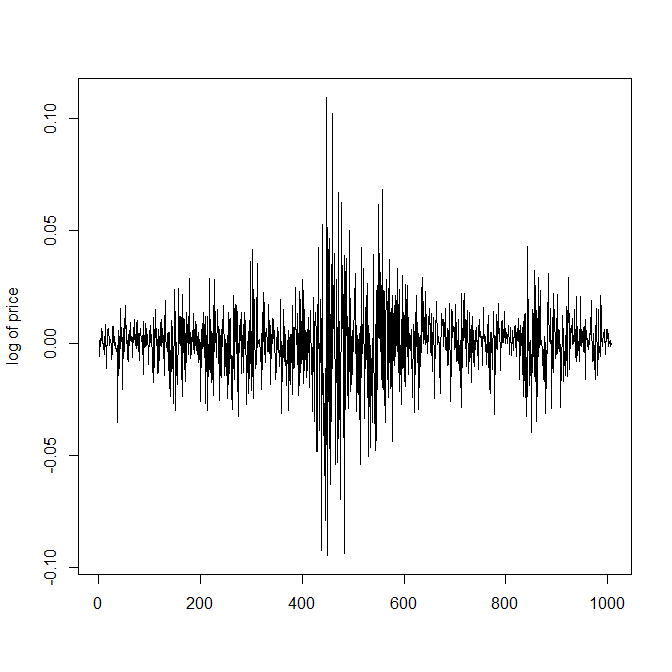
\includegraphics[scale=0.3]{sp}
\caption{Daily change of S$\&$P500 closing price from 2007-2010}\label{9}
\end{figure}
\subsection{Result}
We fit model for the data with five methods: MH random walk with three different "speed" $e$, and the other two methods. We will address them as "MH $+$ RW with $e=\dots$", "MH $+$ RA", "RA", respectively. For prior we take $\delta\sim N(0,10)$, $\alpha\sim N(0,10)$ and $\sigma_\nu^2\sim IG(\frac{1}{2},\frac{1}{2})$. We simulate the MCMC for 12000 iterations, and all the posterior results are based on the sample collected after 4000th iteration. We list the result of parameters in Table $\ref{2}$. The numbers outside and inside bracket are posterior mean and standard deviations respectively. From Figure $\ref{3}$ to $\ref{4}$ we give all histograms of these variables. For each $h_t$, we compute its sample mean and plot the log of the mean in Figure $\ref{5}$

\begin{table}
\centering
\begin{tabular}{|c|c|c|c|c|c|c|}
\hline
Method& $\delta$ & $\alpha$& $\sigma_\nu^2$& $Cov(\delta,\alpha)$& $Cov(\delta,\sigma_\nu^2)$&$Cov(\alpha,\sigma_\nu^2)$  \\
&&&&$(\times 10^{-4})$&($\times 10^{-4})$&$(\times 10^{-4})$\\
\hline
MH $+$RW, $e=0.05$ & 0.976(0.008) & -0.214(0.073) & 0.06(0.012) &5.9&-0.12& -1.18 \\
\hline
MH $+$RW,$e=0.1$& 0.977(0.008) &  -0.199(0.067) & 0.061(0.009)&5.07&-0.27&-2.3\\
\hline
MH $+$ RW, $e=0.3$ & 0.973(0.009) & -0.24(0.083) & 0.068(0.015)&7.8&-0.83&-7.3\\
\hline
MH $+$ RA &  0.986(0.006) & -0.113(0.051) & 0.029(0.004)&3.1&-0.05&-0.44\\
\hline
RA& 0.974(0.01) & -0.223(0.089) & 0.071(0.017)&8.97&-1&-8.9\\
\hline
\end{tabular}
\caption{Results of fitting SV model on S$\&$P500 daily log change}\label{2}
\end{table}
\begin{figure}
\centering
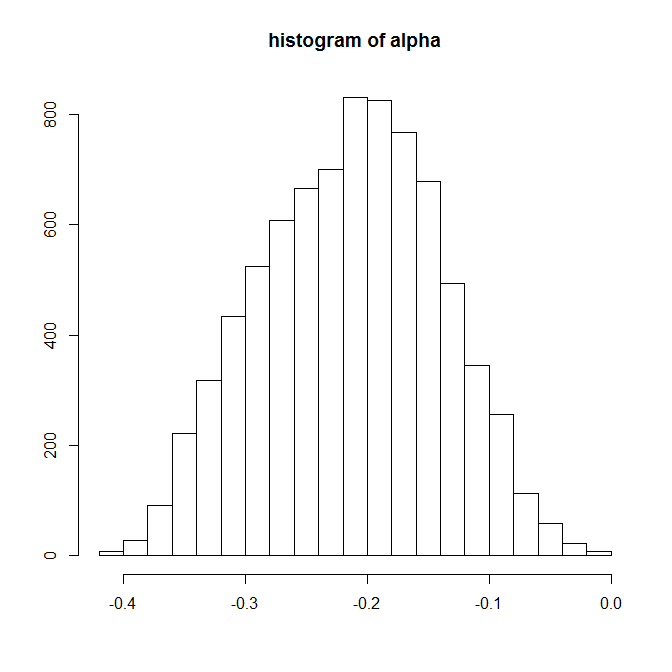
\includegraphics[scale=0.2]{hmrw1halpha}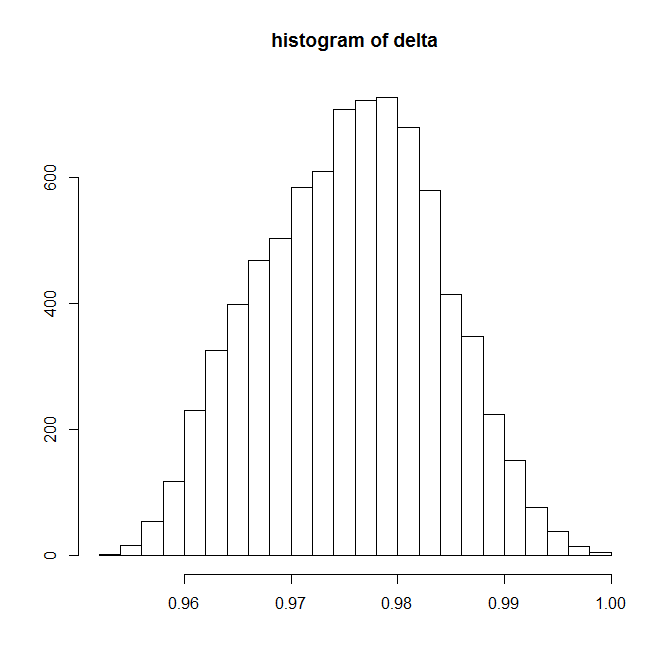
\includegraphics[scale=0.2]{hmrw1hdelta}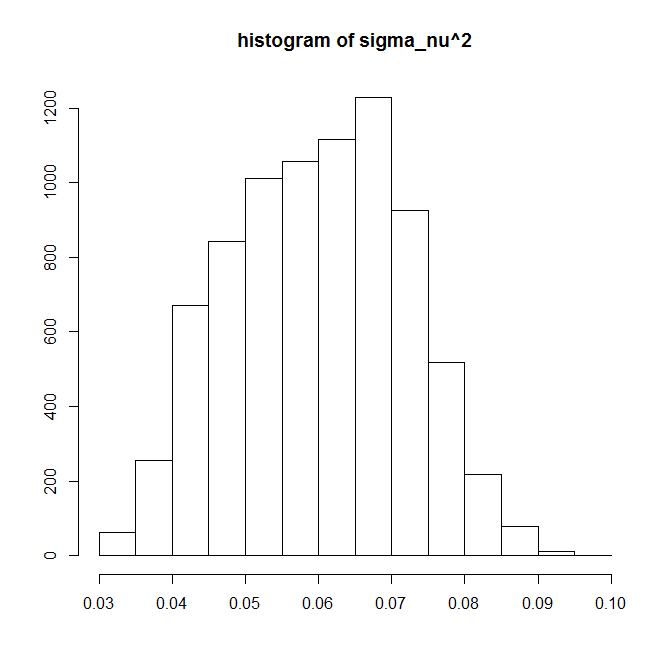
\includegraphics[scale=0.2]{hmrw1hsig}
\caption{Histograms of MH $+$ RW with $e=0.05$}\label{3}
\end{figure}
\begin{figure}
\centering
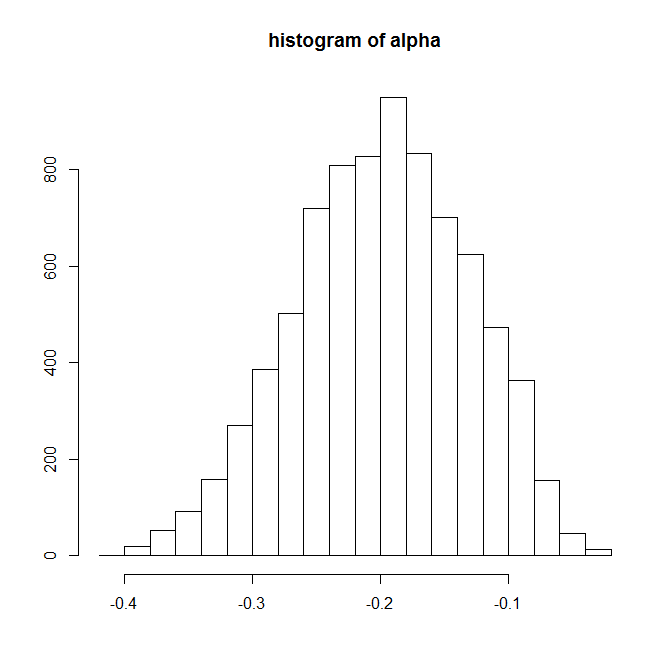
\includegraphics[scale=0.2]{hmrw2halpha}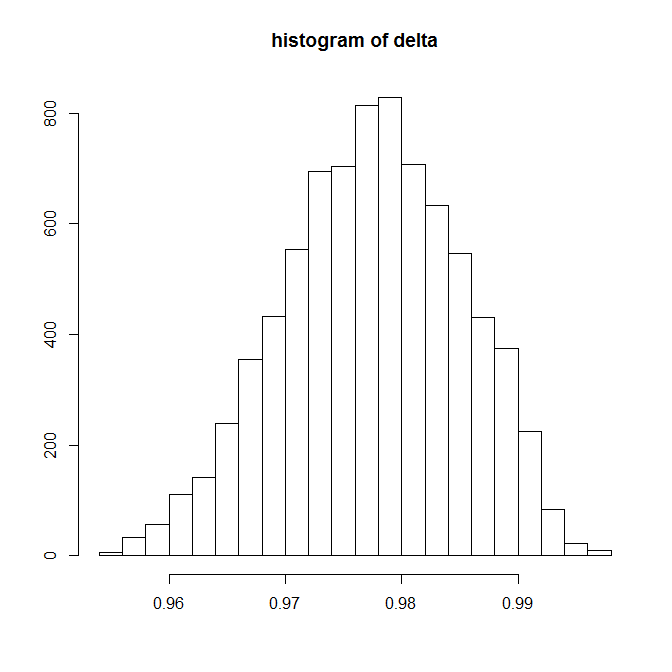
\includegraphics[scale=0.2]{hmrw2hdelta}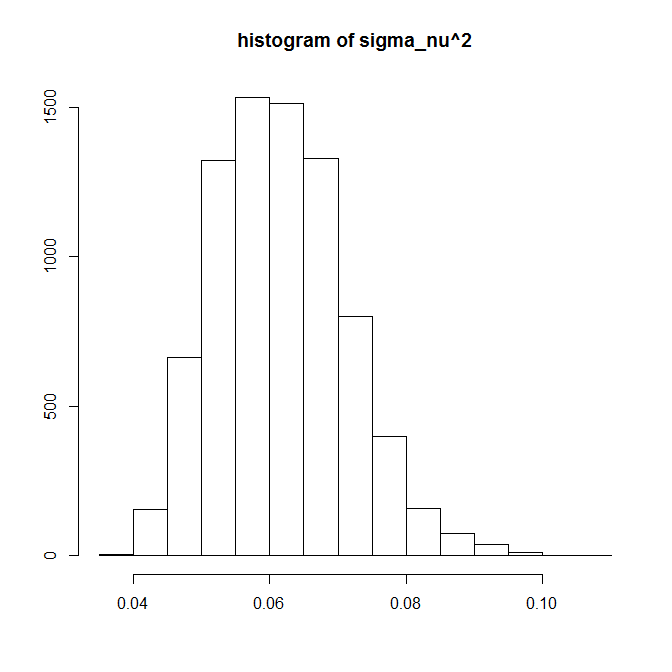
\includegraphics[scale=0.2]{hmrw2hsig}
\caption{Histograms of MH $+$ RW with $e=0.1$}
\end{figure}
\begin{figure}
\centering
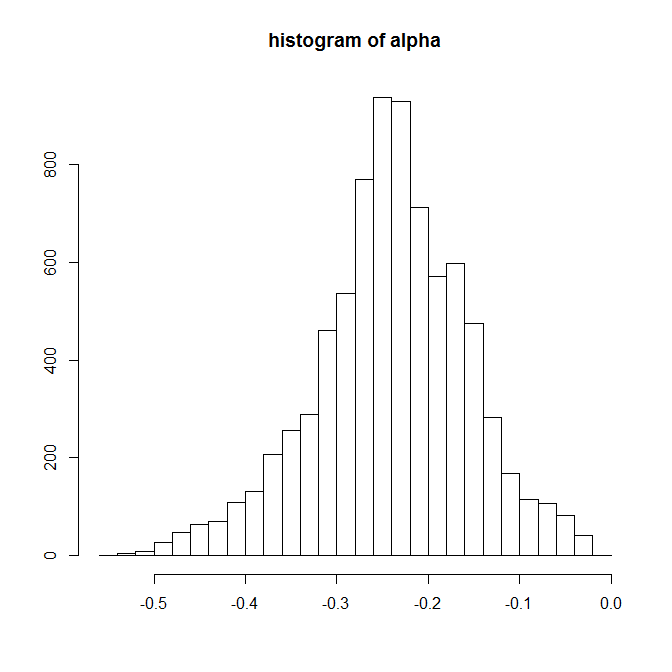
\includegraphics[scale=0.2]{hmrw3halpha}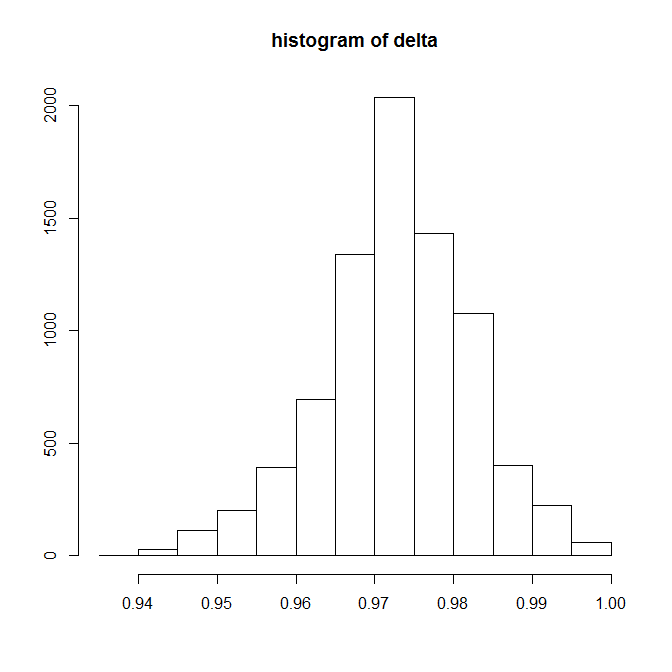
\includegraphics[scale=0.2]{hmrw3hdelta}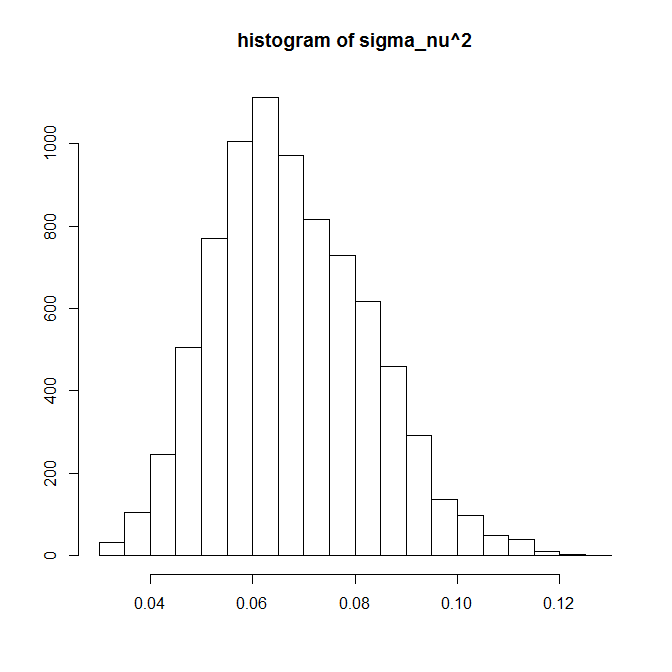
\includegraphics[scale=0.2]{hmrw3hsig}
\caption{Histograms of MH $+$ RW with $e=0.3$}
\end{figure}
\begin{figure}
\centering
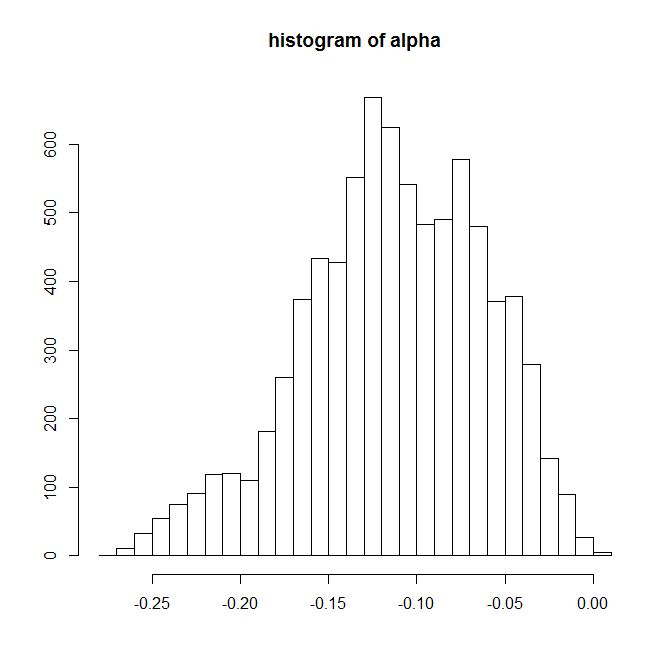
\includegraphics[scale=0.2]{hmrahalpha}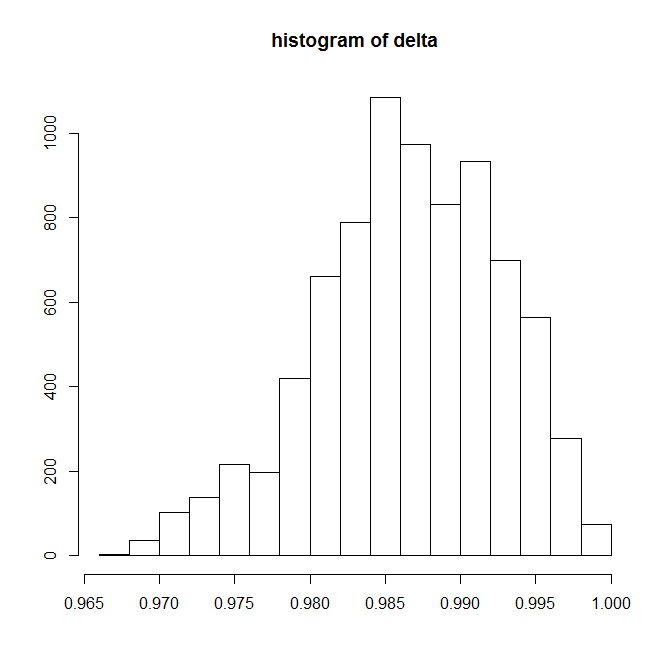
\includegraphics[scale=0.2]{hmrahdelta}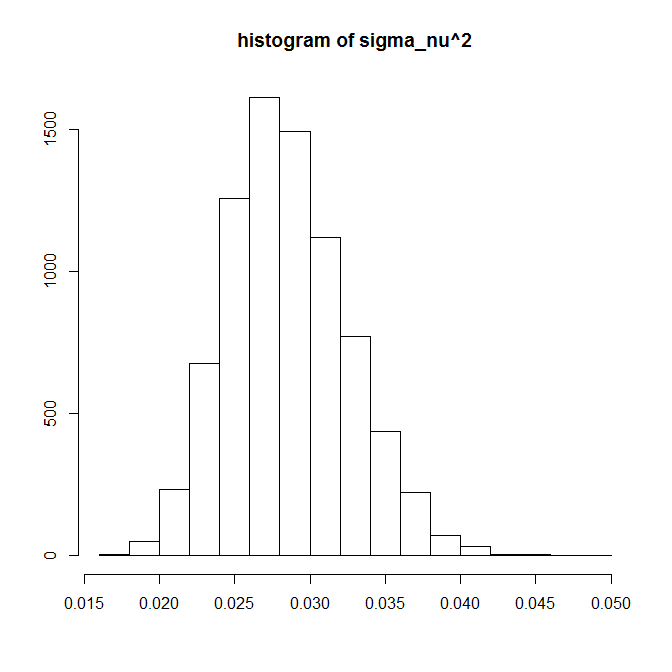
\includegraphics[scale=0.2]{hmrahsig}
\caption{Histograms of MH $+$ RA}
\end{figure}
\begin{figure}
\centering
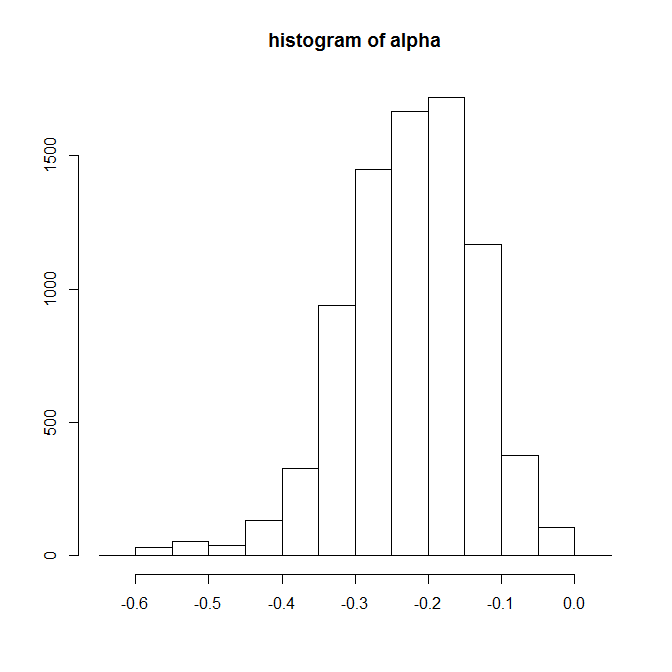
\includegraphics[scale=0.2]{rahalpha}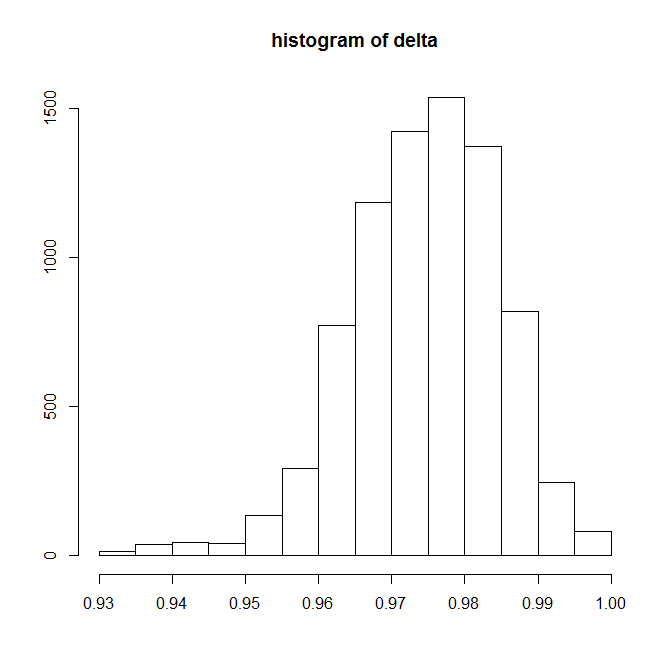
\includegraphics[scale=0.2]{rahdelta}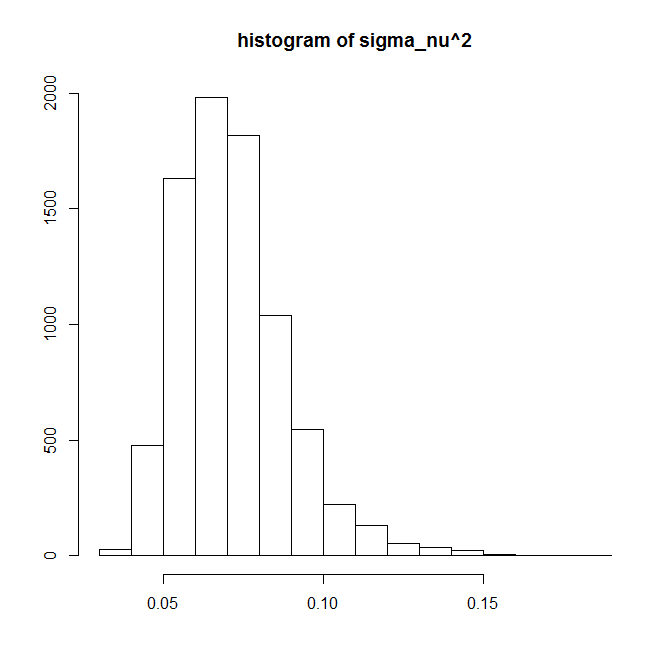
\includegraphics[scale=0.2]{rahsig}
\caption{Histograms of RA}\label{4}
\end{figure}

\begin{figure}
\centering
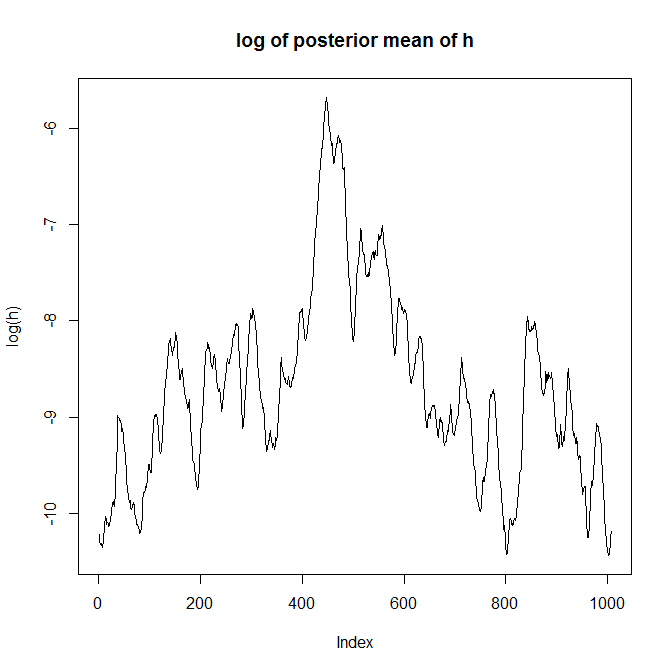
\includegraphics[scale=0.2]{hmrw1h}
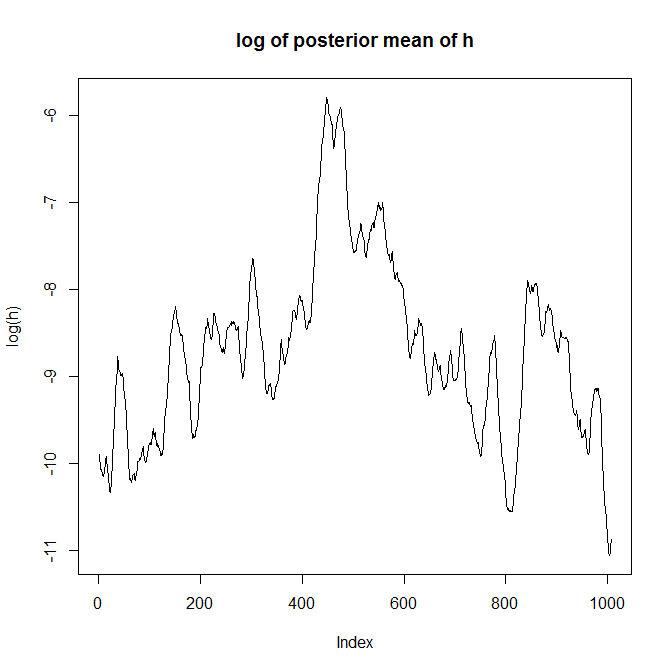
\includegraphics[scale=0.2]{hmrw2h}
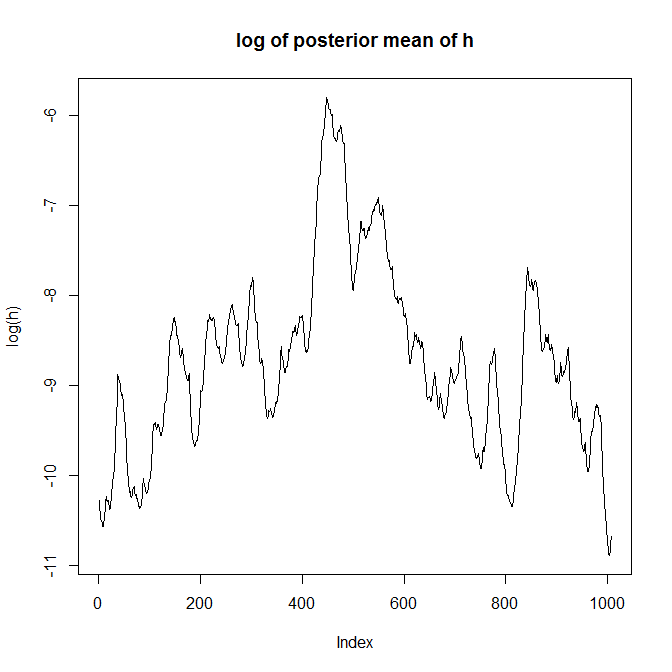
\includegraphics[scale=0.2]{hmrw3h}
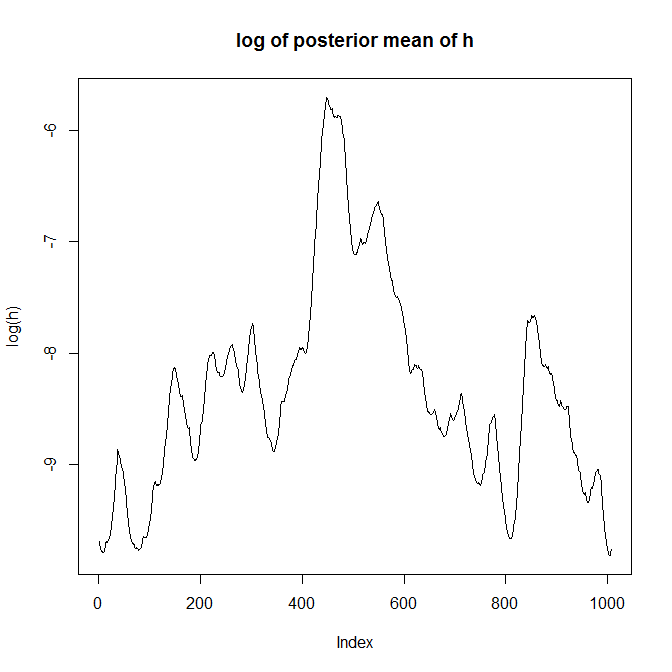
\includegraphics[scale=0.2]{hmrah}
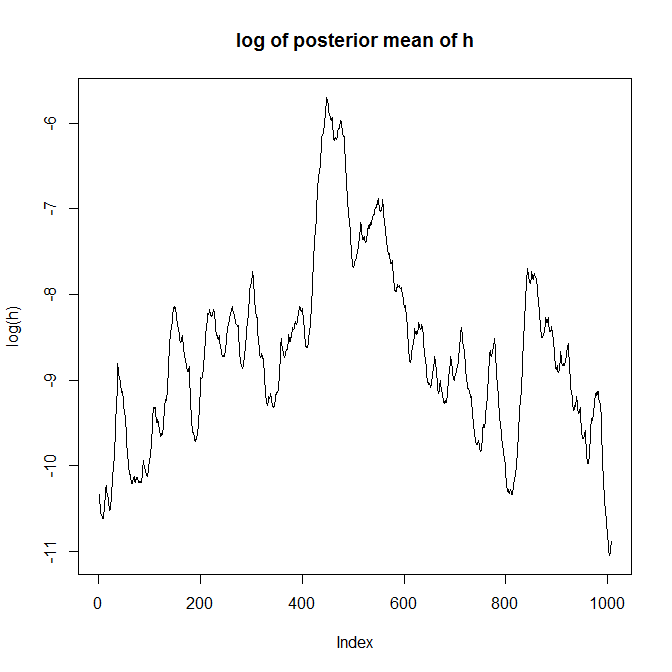
\includegraphics[scale=0.2]{rah}
\caption{Log of mean of $h_t$ of five methods, in the order of appearance in previous tables}\label{5}
\end{figure}
\subsection{Time}
In Table $\ref{6}$  we listed the time and rejection/repeat rate of each method for 12000 iterations. Repeat rate applies for methods involving MH algorithm, while rejection rate applies for methods involving RA sampling. Note that only the HM+RA method have both.
\begin{table}
\begin{tabular}{|c|c|c|c|}
\hline
Method&Time for 12000 iteration (second)& reject rate& repeated rate  \\
\hline
MH $+$ RW, $e=0.05$ & 213.42 &  & 0.1\\
\hline
MH $+$ RW, $e=0.1$&  210.64 &  & 0.18 \\
\hline
MH $+$ RW, $e=0.3$ & 215.87 &  & 0.44\\
\hline
MH $+$RA & 451.58 & 0.09 & 0.0002\\
\hline
RA & 171.39 & 0.008 & \\
\hline
\end{tabular}
\caption{Time and reject/repeat rate of each method}\label{6}
\end{table}
\subsection{Autocorrelation}
We give the autocorrelation function of parameters fit by all methods in Figure $\ref{7}$ to $\ref{8}$. The autocorrelation function are computed and plotted using acf() in stats library of R.
\begin{figure}
\centering
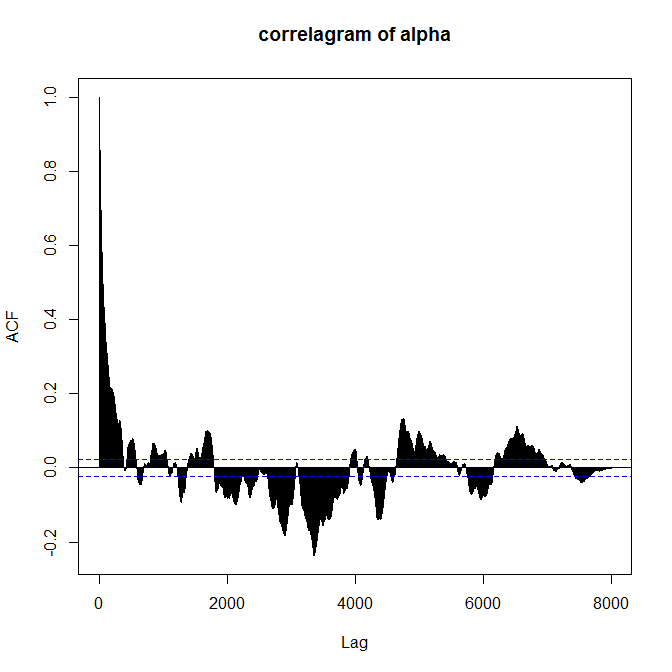
\includegraphics[scale=0.2]{corhmrw1alpha}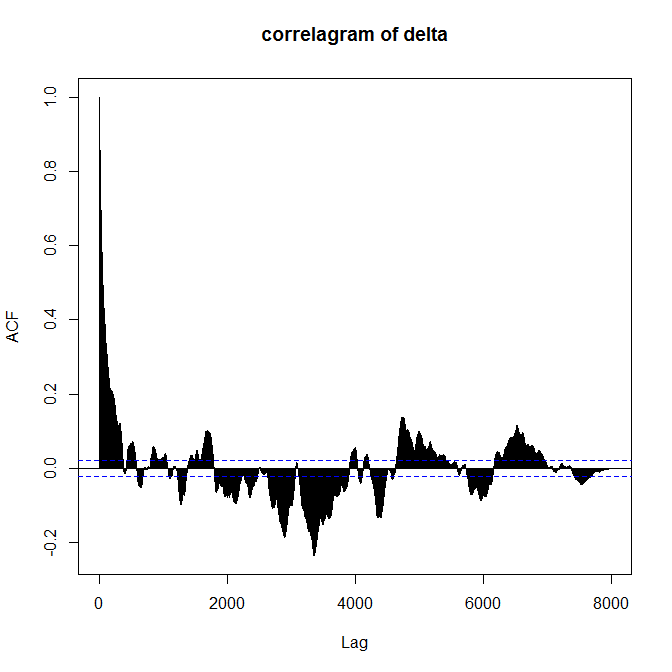
\includegraphics[scale=0.2]{corhmrw1delta}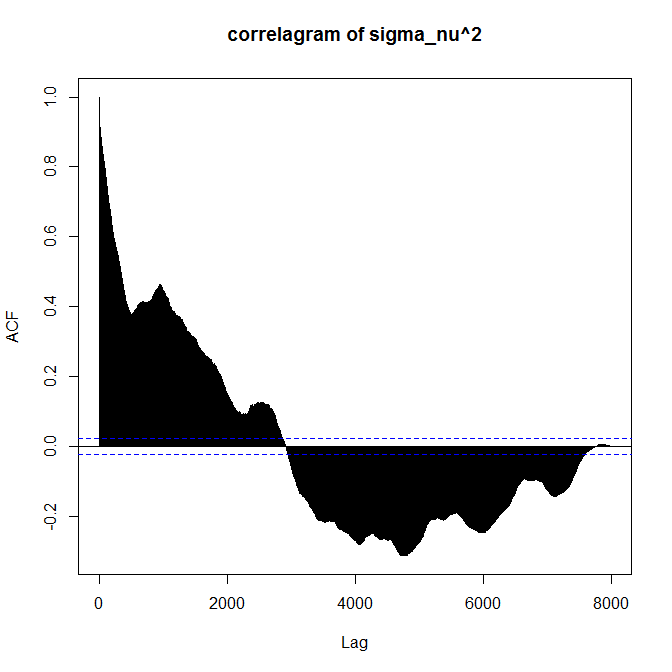
\includegraphics[scale=0.2]{corhmrw1sig}
\caption{Correlagram of MH $+$ RW with $e=0.05$}\label{7}
\end{figure}
\begin{figure}
\centering
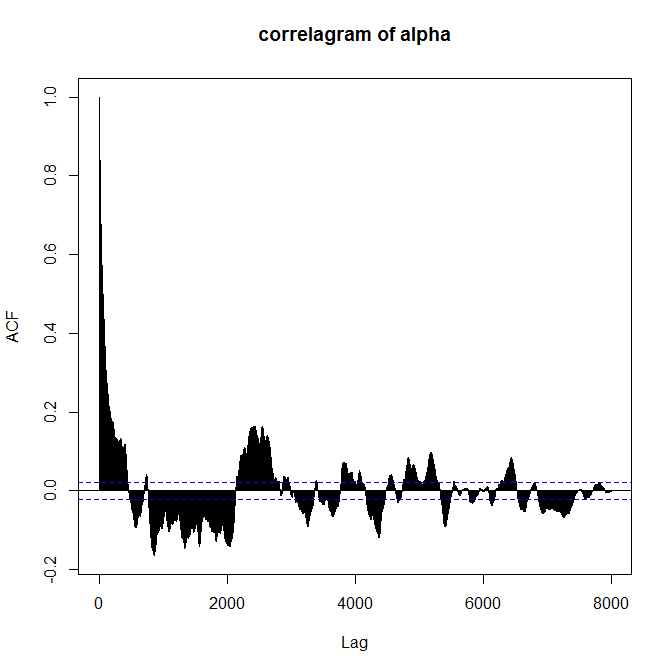
\includegraphics[scale=0.2]{corhmrw2alpha}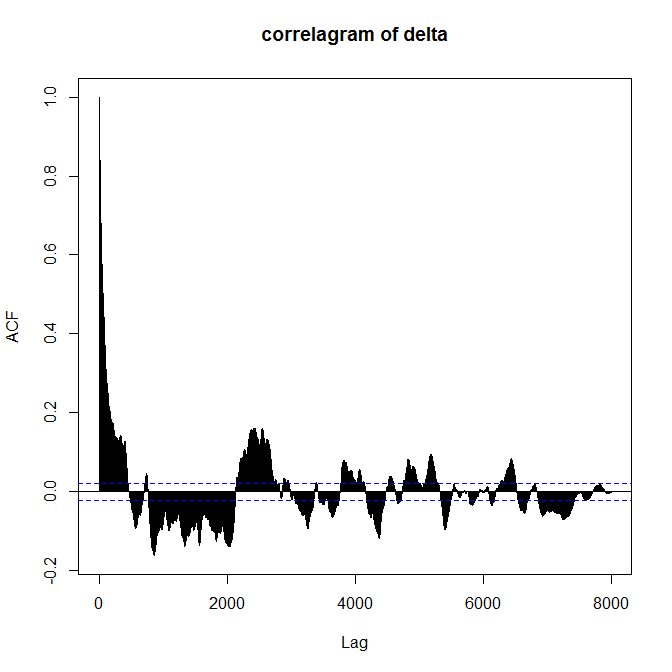
\includegraphics[scale=0.2]{corhmrw2delta}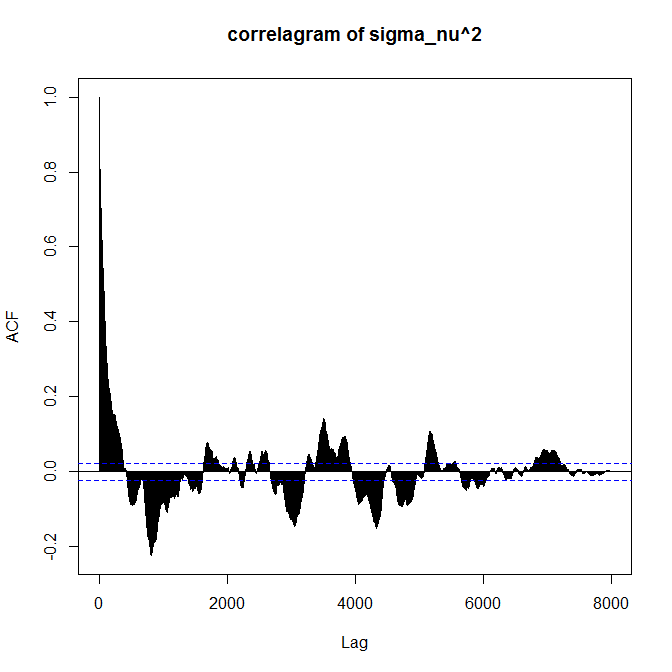
\includegraphics[scale=0.2]{corhmrw2sig}
\caption{Correlagram of MH $+$ RW with $e=0.1$}
\end{figure}
\begin{figure}
\centering
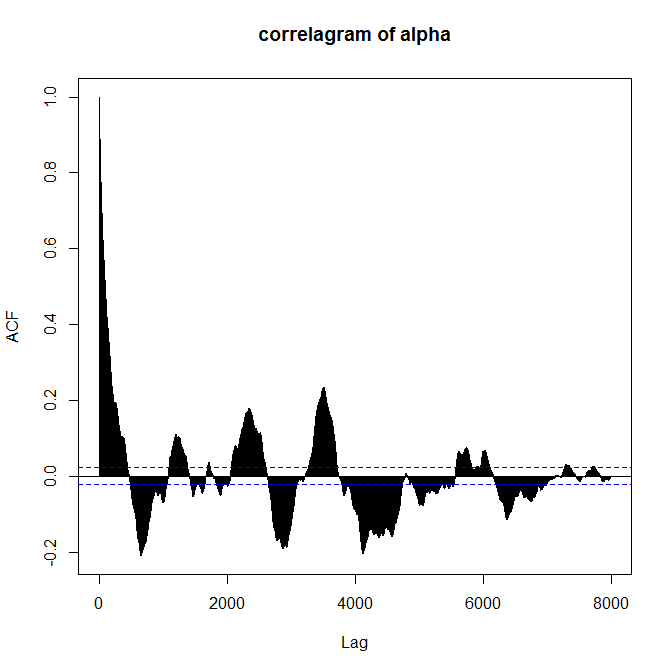
\includegraphics[scale=0.2]{corhmrw3alpha}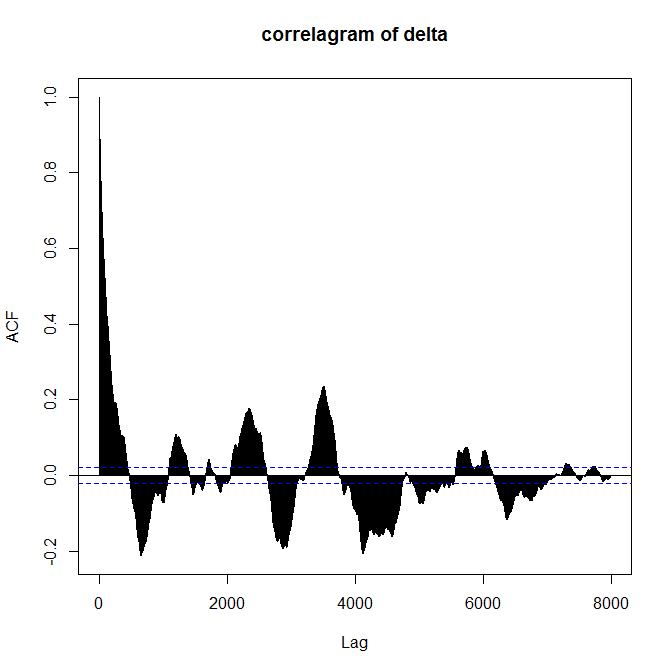
\includegraphics[scale=0.2]{corhmrw3delta}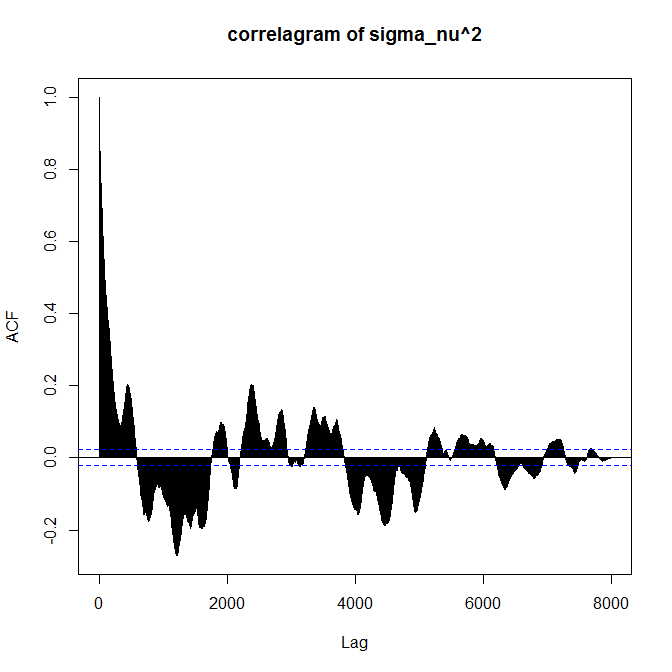
\includegraphics[scale=0.2]{corhmrw3sig}
\caption{Correlagram of MH $+$ RW with $e=0.3$}
\end{figure}
\begin{figure}
\centering
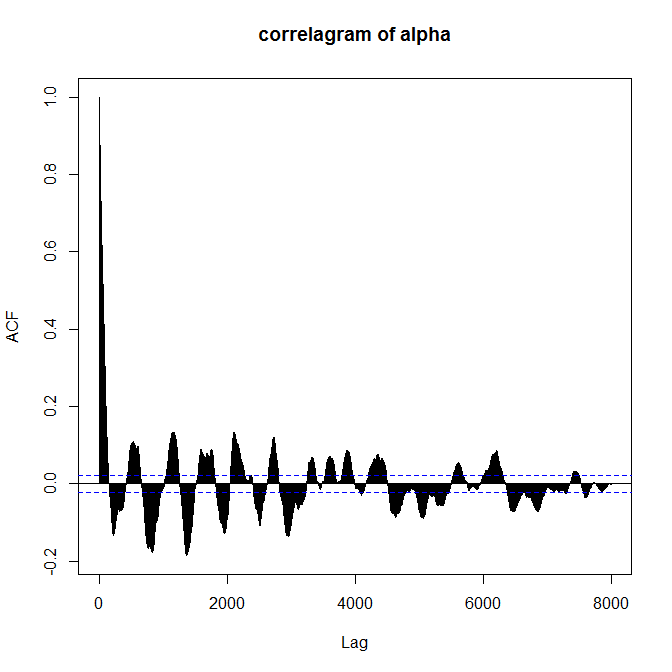
\includegraphics[scale=0.2]{corhmraalpha}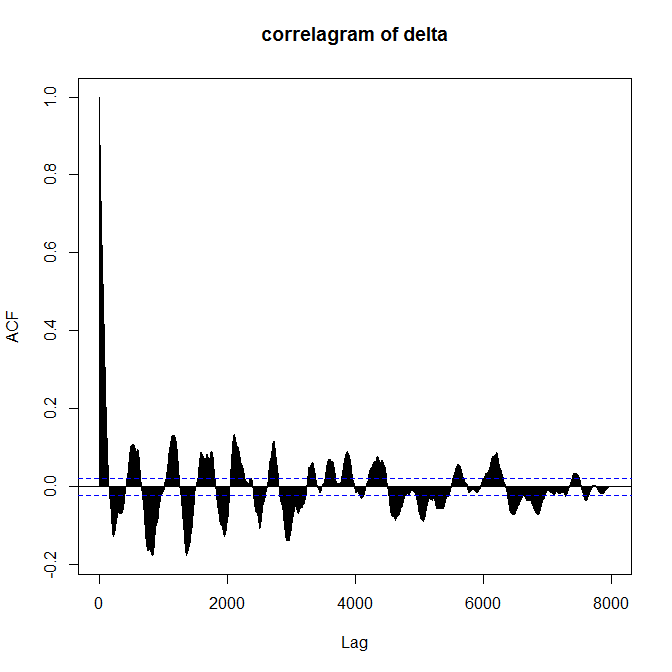
\includegraphics[scale=0.2]{corhmradelta}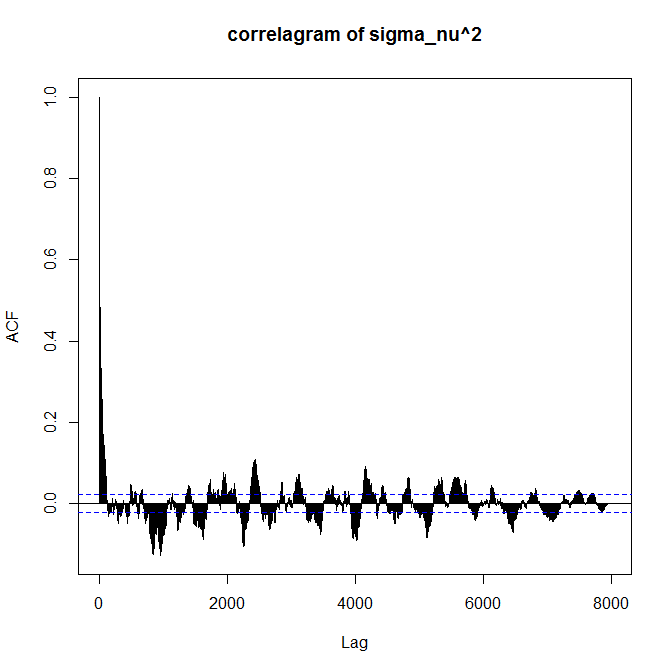
\includegraphics[scale=0.2]{corhmrasig}
\caption{Correlagram of MH $+$ RA}
\end{figure}
\begin{figure}
\centering
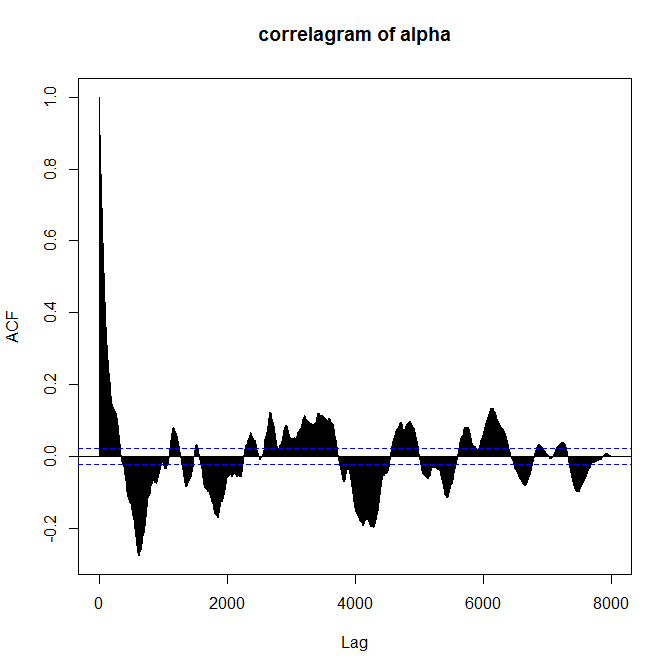
\includegraphics[scale=0.2]{corraalpha}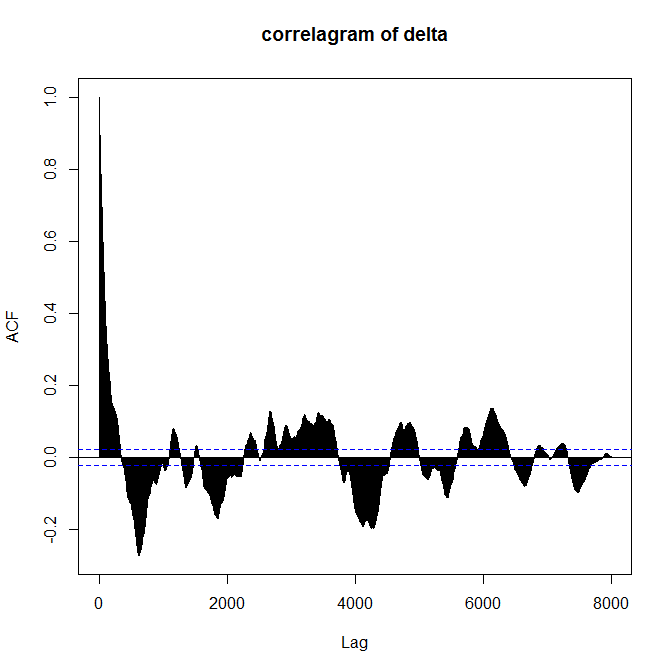
\includegraphics[scale=0.2]{corradelta}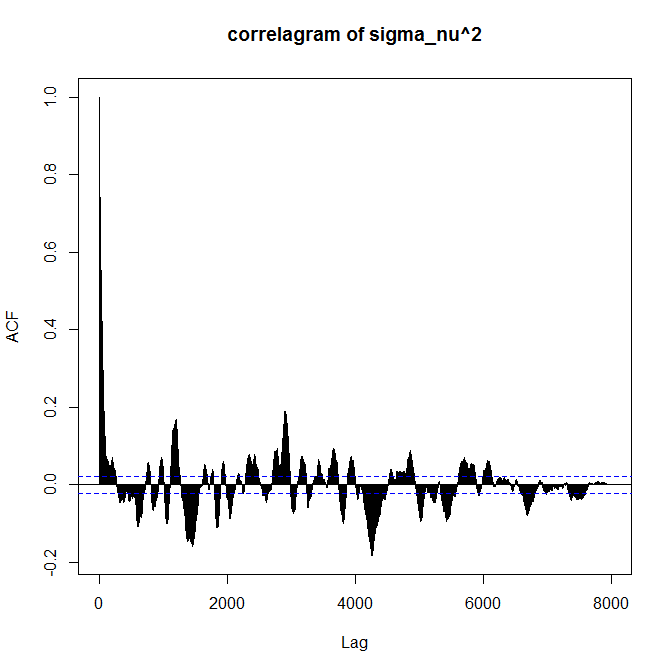
\includegraphics[scale=0.2]{corrasig}
\caption{Correlagram of RA}\label{8}
\end{figure}
\section{Comparison with GARCH}
\subsection{Data}
We will use multiple data in this section: S$\&$P500, Nasdaq composite and Nikkei 225. 
\section{Reference}
\begin{enumerate}
\item
Eric Jacquier, Nicholas G. Polson and Peter E. Rossi, "Bayesian Analysis of Stochastic Volatility Models", Journal of Business $\&$ Economic Statistics, 1994, Vol. 12, No. 4
\item
Eric Jacquier, Nicholas G. Polson and Peter E. Rossi, "Bayesian analysis of stochastic volatility models with fat-tails and correlated errors", Journal of Econometrics, 122(2004) 185-212
\item
John Geweke, "Prior for Macroeconomic Time Series and Their Application", Econometric Theory, Vol. 10, 609-632
\item
John Geweke, "Bayesian Comparison of Econometric Models", working paper, Federal Reserve Bank of
Minneapolis Research Department
\item
Siddhartha Chib and Edward Greenberg, "Understanding the Metropolis-Hastings Algorithm", The American Statistician, Vol. 49, No. 4. (Nov., 1995), pp.327-335
\item
A. Ronald Gallant, Peter E. Rossi, George Tauchen, "Stock Prices and Volume", The Revew of Financial Studies, Vol. 5, No. 2. (1992), pp. 199-242
\item
Sangjoon Kim, Neil Shephard, Siddhartha Chib, "Stochastic Volatility: Likelihood Inference and Comparison with ARCH Model", Review of Economic Studies (1998) 65, 361-393
\end{enumerate}
\end{document}